% =============================================================================
% Evaluation
% =============================================================================

\section{Evaluation}
\label{sec:evaluation}

We evaluate three questions on natural Claude Code (CC) traffic:
(i) does \sys{} actually rescue post-compaction tokens at the rate the
underlying cacheblend mechanism is claimed to (\S\ref{sec:eval-hitrate});
(ii) does cacheblend's blended-KV output match a full-compute baseline
bit-for-bit at temperature~0 (\S\ref{sec:eval-identity}); and (iii) when
it does not, is the divergent output of equal quality to the baseline
under a strong LLM judge (\S\ref{sec:eval-judge}). The first two
questions admit numerical answers; the third governs deployment
viability.

\paragraph{Methodology.} The backend is Llama-3.3-70B-Instruct fp8 on
2$\times$ NVIDIA H100 80GB in tensor-parallel mode (TP=2), with
vLLM v0.19.0 and lmcache v0.4.2 patched per \S\ref{sec:patches}
(\texttt{max\_model\_len}=32768, \texttt{LMCACHE\_BLEND\_RECOMPUTE\_RATIOS}
=0.15 default). The replay corpus is \dataset's
\texttt{swebench\_verified/} subset (5 captures: astropy-13398,
matplotlib-26113, pylint-7080, pytest-7490, sphinx-11510) and the
\texttt{post\_compact/} v6+v7 captures (2 captures, the ones with
$\geq$256-token substantive turns; v1--v5 are diagnostic and excluded).
Together: 7 captures, 54 (capture, turn) pairs total, of which 47 are
substantive ($\geq$256-token prompts) and 7 are preflight pings.

For each (capture, turn), we replay the captured request body through
the proxy under three conditions:

\begin{description}
\item[\textbf{no\_cache}] vLLM prefix caching disabled, lmcache
  inactive. The all-fresh-compute baseline.
\item[\textbf{prefix\_cache}] vLLM paged-attention prefix caching
  enabled, lmcache inactive. Should be mathematically equivalent to
  no\_cache when no prior cross-request state exists.
\item[\textbf{cacheblend}] lmcache enabled with our patches, cacheblend
  blending active. The condition under test.
\end{description}

We compute token-identity via longest common prefix over each output's
token sequence, normalized by the longer length. All measurements are
at $T=0$, $N{=}1$ sample per condition. The 7 preflight turns under
lmcache's \texttt{blend\_min\_tokens}=256 cutoff bypass cacheblend
entirely; we exclude them from all identity and preference statistics.

\paragraph{All three conditions receive identical rewritten prompts.}
The CC-segment parser (\S\ref{sec:cc-segment}) and header normalizer
(\S\ref{sec:header-norm}) run inside the proxy unconditionally for
every outbound request --- they are not gated by the cacheblend
backend. The \texttt{no\_cache} and \texttt{prefix\_cache} conditions
therefore see exactly the same prompt bytes as \texttt{cacheblend};
no\_cache simply does not exploit the chunks the parser annotates,
and prefix\_cache hits on exact-prefix chunks but not on
positionally-shifted ones. Any identity gap between
\texttt{no\_cache} and \texttt{cacheblend} is therefore attributable
to the lmcache blending mechanism on shared input, not to different
input text. The header-normalization sanity check
(\S\ref{sec:header-norm}: NC output is bit-identical at $T{=}0$
across all 54 normalized-vs-unnormalized pairs) verifies this
empirically for the header rewrite specifically; the same property
follows analytically for separator injection because vLLM's
tokenizer treats the injected \texttt{\textquotedbl{}~\#~\#~\textquotedbl{}}
as ordinary content tokens whose KV is recomputed deterministically
in the \texttt{no\_cache} condition.

\paragraph{Denominators used in this section.} To keep the reported
percentages unambiguous, every rate in \S\ref{sec:evaluation} is
reported against one of these three denominators:

\begin{itemize}
\item $n_{\text{total}}{=}54$ — every (capture, turn) pair in the
  corpus. Used only for the methodology description; \emph{no
  evaluation rate uses this denominator}.
\item $n_{\text{sub}}{=}47$ — substantive pairs with prompt $\geq$256
  tokens (excluding 7 preflight turns where cacheblend's
  \texttt{blend\_min\_tokens} guard prevents engagement). Used for
  rescue rate (\S\ref{sec:eval-hitrate}), token-identity
  (\S\ref{sec:eval-identity}), tool-call mode agreement
  (\S\ref{sec:eval-mode}), and the \emph{end-to-end} non-inferiority
  rate in \S\ref{sec:eval-judge}.
\item $n_{\text{div}}{=}19$ — the substantive pairs whose
  \texttt{no\_cache} and \texttt{cacheblend} outputs were not
  bit-identical (the other 28 substantive pairs would have returned
  trivial EQUIVALENT). Used for the LLM-judge preference rate and the
  \emph{conditional} non-inferiority rate in \S\ref{sec:eval-judge}.
\end{itemize}

Preflight turns are excluded from every reported rate. We do not
report any rate against a $/54$ denominator; the 54 figure exists only
to account for the corpus breakdown.

\paragraph{Evaluation matrix.} Table~\ref{tab:eval-matrix} maps each
measurement to the corpus subset it was run on. Latency, judge
preference, tool-call mode, and the recompute-ratio sweep were
measured on the SWE-V+\texttt{post\_compact} subset only;
rescue rate and output identity were additionally replicated on
\texttt{skill\_invocation/} (\S\ref{sec:eval-cross-corpus}). Multi-judge
replication used the same divergent slice as the single-judge
analysis.

\begin{table*}[t]
\small
\centering
\begin{tabular}{lcc}
\toprule
Measurement & SWE-V+\texttt{post\_compact} ($n_{\text{sub}}{=}47$) & \texttt{skill\_invocation/} ($n_{\text{sub}}{=}52$) \\
\midrule
Rescue rate (\S\ref{sec:eval-hitrate})                       & \checkmark & \checkmark \\
TTFT latency (\S\ref{sec:eval-latency})                      & \checkmark & --- \\
Output identity (\S\ref{sec:eval-identity})                  & \checkmark & \checkmark \\
LLM-judge preference, single (\S\ref{sec:eval-judge})        & \checkmark ($n_{\text{div}}{=}19$) & --- \\
LLM-judge replication, 3 judges (\S\ref{sec:eval-judge})     & \checkmark ($n_{\text{div}}{=}19$) & --- \\
Tool-call mode agreement (\S\ref{sec:eval-mode})             & \checkmark & --- \\
Recompute-ratio sweep (\S\ref{sec:disc-knobs})               & 3-turn sub-fixture per ratio & --- \\
\bottomrule
\end{tabular}
\caption{Measurement coverage. Rescue rate and output identity
replicate across both subsets
(\S\ref{sec:eval-cross-corpus},~Table~\ref{tab:cross-corpus}); the
remaining measurements use the SWE-V+\texttt{post\_compact} subset
only. Recompute-ratio used a 3-turn sub-fixture (\texttt{pytest-7490})
per ratio.}
\label{tab:eval-matrix}
\end{table*}

\subsection{Hit rate: bimodal, median 87\% across the corpus}
\label{sec:eval-hitrate}

We measure cacheblend's prefill-token rescue rate per turn across all
$n{=}47$ substantive turns of the SWE-V+\texttt{post\_compact} subset, joining the per-request
\texttt{LMCache hit tokens} accounting in \texttt{vllm.log} to the
parquet of model outputs on the OpenAI \texttt{response\_id}. Rescue
rate for a turn is defined as \texttt{hit\_tokens} divided by
\texttt{total\_prompt\_tokens}.

\begin{table}[t]
\small
\centering
\begin{tabular}{lr}
\toprule
Statistic over the 47 substantive turns & Rescue \% \\
\midrule
Mean             & 63.6\% \\
\textbf{Median}  & \textbf{87.5\%} \\
25th percentile  & 16.1\% \\
75th percentile  & 96.8\% \\
\midrule
Turns with rescue $\geq 99\%$ (steady-state) & 6/47 (13\%) \\
Turns with rescue $\geq 95\%$               & 15/47 (32\%) \\
Turns with rescue $\geq 80\%$               & 28/47 (60\%) \\
Turns with rescue $< 50\%$                  & 16/47 (34\%) \\
\textbf{Turns with rescue $\approx$ 0\% (cold-cache)} & \textbf{9/47 (19\%)} \\
\bottomrule
\end{tabular}
\caption{Cacheblend rescue rate distribution across the
SWE-V+\texttt{post\_compact} subset (47 substantive turns; 7
preflight turns at $<$256 prompt
tokens are excluded). \emph{The distribution is bimodal} ---
the mean and median diverge by 24 points because a 19\% mass of
cold-cache turns at $\sim$0\% rescue pulls the mean down, while the
upper quartile sits near the published rescue peak.}
\label{tab:hit-rate}
\end{table}

\begin{figure}[t]
\centering
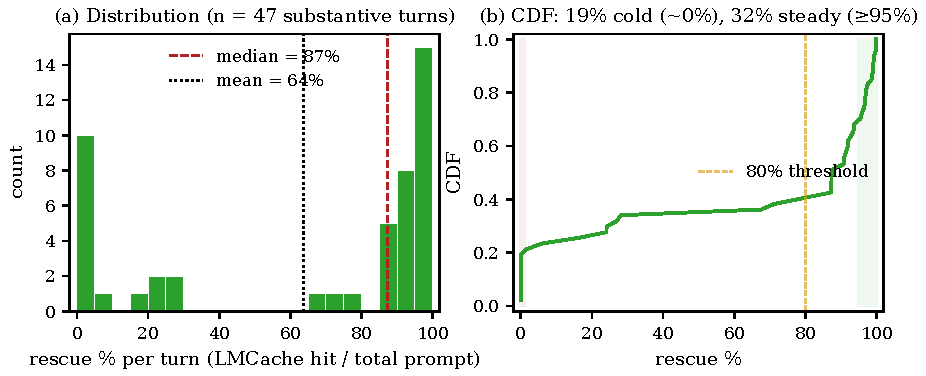
\includegraphics[width=\columnwidth]{figures/rescue_distribution.pdf}
\caption{Per-turn rescue rate across the 47 substantive turns.
\textbf{(a)} Histogram with median and mean overlaid: the bimodality
is sharp --- a mass near 0\% (cold-cache first-turns of each capture
plus pattern-shift turns where cacheblend's LOOKUP cannot find a
match) and a steady-state peak above 90\%. \textbf{(b)} CDF: 19\% of
turns rescue near 0\%, 32\% reach $\geq$95\%, the rest are distributed
across the intermediate band.}
\label{fig:rescue-distribution}
\end{figure}

\paragraph{Two regimes.} Table~\ref{tab:hit-rate} and
Figure~\ref{fig:rescue-distribution} reveal two regimes with sharply
different rescue behavior. In the \emph{steady-state regime}
(post-cache-warmup turns of a session repeating a stable prompt
pattern), cacheblend rescues 95--99\% of prefill tokens, matching
the published cacheblend headline. In the \emph{cold/shift regime}
(the first turn of any capture, or a subsequent turn whose prompt
shifts in a way cacheblend's LOOKUP cannot match) the mechanism
fires zero or near-zero rescue. Within the SWE-V+\texttt{post\_compact} subset these two
regimes split roughly 60/40 in favor of steady-state.

\paragraph{Cross-fixture comparison.} The 95--99\% steady-state
numbers were first reported on a minimum-effective fixture
(\texttt{swebench\_verified/\allowbreak{}pytest-7490}, 4 turns, samples=2)
during patch development and are reproduced here at the top of the
per-fixture rescue distribution. Generalizing those
numbers to the full SWE-V+\texttt{post\_compact} subset shows that the steady-state peak is
real, but a roughly equal-sized cold/shift tail accompanies it ---
a structural property of the cacheblend mechanism on this workload,
not a calibration artifact. The next two sections measure what
happens when rescue \emph{does} engage.

\subsection{Latency: cacheblend is slower than no\_cache in every rescue regime}
\label{sec:eval-latency}

The hit-token rescue rate of \S\ref{sec:eval-hitrate} is an
\emph{intermediate} metric. The deployment-facing measurement is
end-to-end TTFT (time-to-first-token). For each (capture, turn,
condition) tuple, the bench harness recorded the SDK-reported
\texttt{ttft\_ms}; we summarize per condition over the 47 substantive
turns:

\begin{table}[h]
\small
\centering
\begin{tabular}{lrrrr}
\toprule
Condition & p25 & median & p75 & p95 \\
\midrule
\texttt{no\_cache}      & 1028 ms & \textbf{1211 ms} & 1473 ms & 8660 ms \\
\texttt{prefix\_cache}  & 994 ms  & 1261 ms          & 1476 ms & 8739 ms \\
\texttt{cacheblend}     & 1528 ms & \textbf{1882 ms} & 3520 ms & 9187 ms \\
\bottomrule
\end{tabular}
\caption{TTFT distribution per condition on the 47 substantive turns
of the SWE-V+\texttt{post\_compact} subset. \texttt{prefix\_cache} is statistically
indistinguishable from \texttt{no\_cache} at this corpus size (lookup
overhead is in the noise floor). \texttt{cacheblend}'s median TTFT
is \emph{55\% larger} than \texttt{no\_cache}'s.}
\label{tab:ttft}
\end{table}

\paragraph{The slowdown is largest at peak rescue.} Bucketing the 47
substantive turns by their cacheblend rescue rate
(Table~\ref{tab:hit-rate}) shows that the TTFT cost is not paid only on
cold-cache turns; it is paid most aggressively on the steady-state
high-rescue turns where the published cacheblend numbers shine:

\begin{table}[h]
\small
\centering
\begin{tabular}{lrrrr}
\toprule
Rescue regime & $n$ & NC median & CB median & Speedup \\
\midrule
Cold ($<$1\% rescue)         & 9  & 1190 ms & 1157 ms & \textbf{1.00$\times$} \\
Mid (1--80\%)                & 10 & 1267 ms & 1948 ms & 0.69$\times$ \\
Hot ($\geq$80\%)             & 28 & 1157 ms & 1930 ms & 0.67$\times$ \\
\midrule
\emph{Peak} ($\geq$95\%)     & 15 & 1068 ms & 2103 ms & 0.50$\times$ \\
\emph{Peak} ($\geq$99\%)     & 6  & 1037 ms & 7342 ms & \textbf{0.12$\times$} \\
\bottomrule
\end{tabular}
\caption{TTFT speedup of \texttt{cacheblend} relative to
\texttt{no\_cache}, bucketed by per-turn rescue rate.
\textbf{Latency cost scales with rescue}: the turns where cacheblend
rescues the most prefill tokens (95--99\% hit rate) are also the
turns where it pays the largest end-to-end latency cost. On the 6 turns reaching $\geq$99\% rescue,
\texttt{cacheblend}'s median TTFT is \emph{7$\times$ larger} than
\texttt{no\_cache}'s.}
\label{tab:ttft-by-rescue}
\end{table}

\paragraph{Where the overhead comes from (hypothesis).} We do not
have an instrumented latency breakdown by phase (LMCache LOAD vs.\
GPU prefill vs.\ recompute pass vs.\ scheduler overhead) and so
report only the end-to-end TTFT above. The qualitative shape of the
result --- cacheblend losing most aggressively at peak rescue, where
LOAD volume is highest --- is consistent with the LMCache LOAD path
(CPU$\to$GPU KV transfer over PCIe plus the selective-recompute
layer pass) being the dominant overhead on this backend. On
2$\times$ H100 80GB SXM, vLLM's batched prefill on Llama-70B fp8 is
fast enough that the per-request prefill cost does not dominate;
LOAD bandwidth is comparatively cheaper to bound. Cacheblend's
published latency wins were measured on different model/hardware
regimes (smaller models where prefill dominates more, slower
interconnect where transfer is relatively cheaper, or aggregate
throughput rather than per-turn TTFT). \emph{We do not claim a
mechanistic explanation; we report the measurement and treat the
phase-breakdown as a resource-constrained gap
(\S\ref{sec:disc-resource}).}

This finding is independent of the agent-protocol cost in
\S\ref{sec:eval-judge}: even if cacheblend's blended output were
\emph{bit-identical} to no\_cache (which we have established it is
not on 30\% of substantive turns), it would still be 55\% slower at
the median and 7$\times$ slower at the peak. On this setup,
hit-token rescue does not translate into TTFT reduction.

\subsection{Output identity: cacheblend's STORE path is bit-identical, LOOKUP path diverges}
\label{sec:eval-identity}

\paragraph{Mathematical equivalence on Llama-70B fp8.} We replay all
54 (capture, turn) pairs at $T=0$ under all three conditions.
\textbf{no\_cache and prefix\_cache produce bit-identical output across
all 54 pairs} (\texttt{token\_identity\_rate}~$=$~1.0000 on 54/54).
Mathematical equivalence on Llama-70B fp8 with our pod configuration is
confirmed at scale --- vLLM's paged-attention prefix caching does not
perturb greedy decoding even when it shortcuts the entire prefix.

\paragraph{Cacheblend diverges on a meaningful fraction.} Cross-condition
no\_cache$\leftrightarrow$cacheblend token-identity is more nuanced.
Across all 47 substantive ($\geq$256-token prompt) turns at $T=0$:

\begin{itemize}
\item Median identity = \textbf{1.0000}, IQR = [0.1088, 1.0000]
\item \textbf{57\%} bit-identical (identity~$\geq$0.9999)
\item 6\% high-but-imperfect (0.7--0.9999)
\item 6\% mid (0.3--0.7) --- typically same tool, different argument
  generation
\item \textbf{30\%} low ($<$0.3) --- severe divergence
\item Including \textbf{11\%} at $\approx$0 identity --- decode-mode
  flips (tool-call $\to$ natural-language prose)
\end{itemize}

The distribution is sharply bimodal (Figure~\ref{fig:identity-distribution}):
either the blended-KV state produces the exact same argmax token-by-token,
or it diverges almost immediately. The middle ground is empirically rare.
Median identity is 1.0000 because more than half of substantive turns
are bit-identical, but the lower quartile at 0.11 places a quarter of
turns near 10\% identity. The bimodality matters: a median-only
reading would mistake this for a $\geq$99\%-identity result, when in
fact the divergence is concentrated in the lower tail.

\begin{figure}[t]
\centering
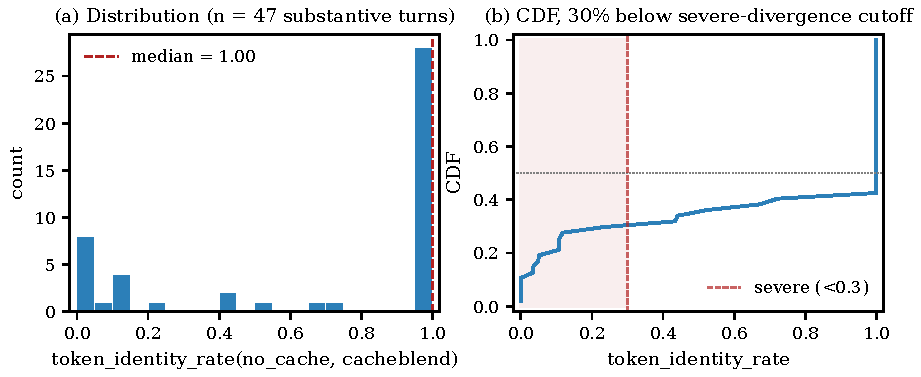
\includegraphics[width=\columnwidth]{figures/identity_distribution.pdf}
\caption{Distribution of \texttt{token\_identity\_rate(no\_cache,
cacheblend)} across 47 substantive ($\geq$256-token prompt) turns at
$T=0$. \textbf{(a)} Histogram: a mass at 1.0 (bit-identical) and a tail
at 0--0.1 (severe divergence). \textbf{(b)} CDF: 30\% of turns fall below
the severe-divergence cutoff at 0.3. The middle bins are empirically rare;
the distribution is sharply bimodal.}
\label{fig:identity-distribution}
\Description{Two-panel figure. Left panel is a histogram of
token-identity rates across 47 substantive turns; bars are concentrated
at 1.0 with a smaller cluster near 0, and a dashed vertical line marks
the median at 1.0. Right panel is the corresponding cumulative
distribution function; the curve rises sharply near 0 and again near 1,
with the region below 0.3 shaded red, labeled as the severe-divergence
cutoff, capturing 30 percent of the mass.}
\end{figure}

\begin{figure}[t]
\centering
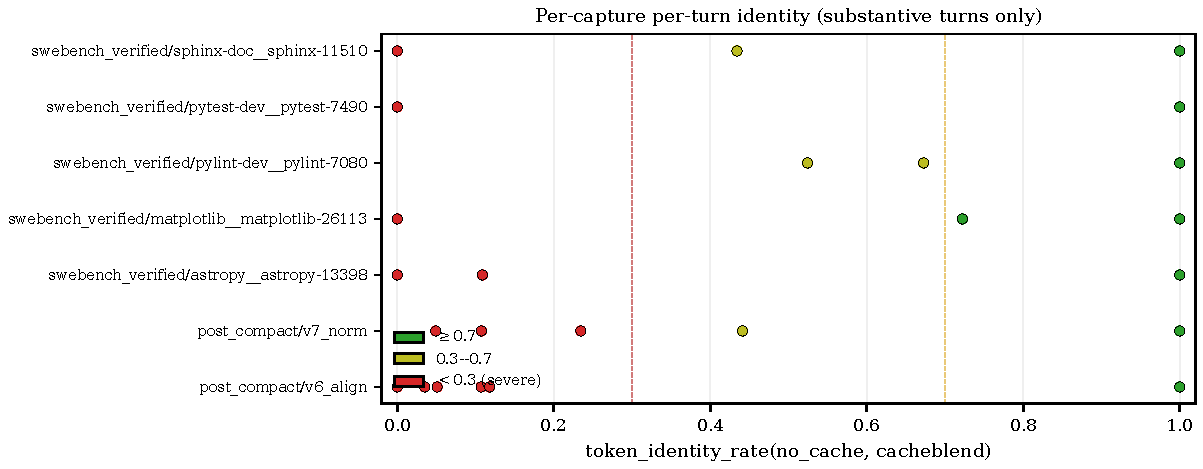
\includegraphics[width=\columnwidth]{figures/per_capture_identity.pdf}
\caption{Per-capture per-turn identity. Each dot is one (capture, turn)
pair, colored by divergence bucket. Severe divergence is not concentrated
in one capture --- every capture in the corpus has at least one turn that
flips below 0.3, indicating the failure mode is generic to the cacheblend
mechanism rather than workload-specific.}
\label{fig:per-capture-identity}
\Description{Strip plot with one row per capture in the corpus. Each
row contains dots representing individual turns, plotted by
token-identity rate on the horizontal axis. Dots below 0.3 are colored
red (severe divergence), between 0.3 and 0.7 yellow, and above 0.7
green. Every capture has at least one red dot, indicating severe
divergence is not concentrated in any single capture.}
\end{figure}

\paragraph{Qualitative shape of the divergence.} Two failure modes
dominate. Mode~A (\emph{severe}, the 30\% tail): the blended-KV state
steers the model away from tool-call mode entirely. On
\texttt{swebench\_verified/pytest-7490} turn~3, the no\_cache output is
a clean 29-token tool-call JSON:
\begin{quote}\small
\texttt{\{"type": "function", "name": "Read", "parameters":
\{"file\_path": "pytest-dev/pytest/pytest.py"\}\}}
\end{quote}
cacheblend's output on the same input is a 362-token natural-language
plan beginning ``\emph{To explore the local code and propose a draft
patch for the issue described in pytest-dev\_\_pytest-7490, we can
follow these steps\dots}''. Both responses are valid; one is what CC's
wire protocol can act on, the other is not. Mode~A is
behavior-changing.

Mode~B (\emph{mild}, the 6\% mid-band): both outputs are tool calls,
both pick the same tool, but the JSON arguments drift. On
\texttt{swebench\_verified/pylint-7080} turn~4, both conditions emit a
\texttt{Bash} tool call with command \texttt{git diff --cached
--name-only}, but cacheblend additionally includes a
\texttt{timeout: "10000"} parameter that no\_cache omits and writes a
different \texttt{description} string. Tool selection preserved;
argument generation drifts. Less downstream-impactful than Mode~A but
still a measurable behavior delta.

The bimodal distribution is inconsistent with the cacheblend paper's
``small but bounded drift'' characterization on this workload: on
Llama-70B fp8 at the default \texttt{recompute\_ratios}=0.15, drift is
concentrated either at zero or in the severe-divergence tail.

\subsection{Agent-protocol usefulness: cacheblend fails non-inferiority on divergent pairs}
\label{sec:eval-judge}

The 30\% severe-divergence tail in Figure~\ref{fig:identity-distribution}
is only a usefulness concern if divergent outputs are also less
task-useful than the no\_cache baseline. The LLM-judge preference
test below isolates this question.

\paragraph{Setup.} We run a blind A/B preference judgment with Sonnet-4.6
on the $n_{\text{div}}{=}19$ substantive pairs whose outputs differed
(of 47 total substantive pairs; the other 28 were trivially equivalent
and would have wasted budget). Position assignment is randomized
(seeded \texttt{rng}{=}42 per pair for reproducibility); prompt-caching
is applied via top-level \texttt{cache\_control} on the static system
prompt. The judge sees the original CC task prompt + both candidate
outputs (labeled A and B) and is asked to return \texttt{PREFER\_A},
\texttt{PREFER\_B}, or \texttt{EQUIVALENT} with a one-sentence rationale.
Outputs are mapped back to \{cacheblend, no\_cache, equivalent\}
via the recorded position assignment.

\paragraph{What the judge measures.} We are not measuring ``output
quality'' in the abstract; we are measuring \emph{next-step usefulness
in a Claude-Code-shaped agent protocol}. The judge prompt
(Appendix~\ref{app:judge-prompt}) is explicit about this calibration ---
it tells the judge that a well-formed tool-call JSON is generally
preferable to natural-language prose, because CC's wire protocol can
only act on tool calls. This is appropriate for an agent-protocol
preference test but not for a generic ``which response is better''
evaluation. We use ``agent-protocol usefulness'' rather than
``output quality'' for the rest of this section to keep the framing
honest.

\paragraph{Result.} Cacheblend's non-inferiority rate on the divergent
slice falls 22 points below the 85\% gate:

\begin{table}[h]
\small
\centering
\begin{tabular}{lrr}
\toprule
Outcome & Count & \% of judged \\
\midrule
Cacheblend wins & 6 & 31.6\% \\
No\_cache wins & 7 & 36.8\% \\
Equivalent & 6 & 31.6\% \\
Unparseable & 0 & 0\% \\
\midrule
\textbf{Cacheblend preference rate} & & \textbf{31.6\%} \\
\textbf{95\% Wilson CI} & & \textbf{[15.4\%, 54.0\%]} \\
\textbf{Non-inferior (wins+ties)} & 12 & \textbf{63.2\%} \\
Non-inferiority gate (spec) & & $\geq$85\% \\
\bottomrule
\end{tabular}
\caption{Sonnet-4.6 blind A/B preference on the $n_{\text{div}}{=}19$
divergent substantive pairs. The 28 substantive pairs with bit-identical
outputs (plus the 7 sub-256-token preflight pairs that bypass cacheblend
entirely) are skipped --- those would all return trivial EQUIVALENT.
Cacheblend's preference rate of 31.6\% with 95\% Wilson CI
[15.4\%, 54.0\%] sits below the no\_cache baseline (36.8\%);
non-inferiority on 63.2\% of the divergent pairs is 22 points short
of the spec gate.}
\label{tab:judge}
\end{table}

\paragraph{Model-family replication.} All three judges below share
Anthropic's RLHF training, so we describe this as
\emph{model-family replication} rather than independent
multi-judge consensus. To check that the
Sonnet-4.6 numbers are not an artefact of a single judge's calibration,
we replicate the same 19-pair blind A/B against Opus-4.7 and Haiku-4.5
with identical prompts and per-pair position assignments:

\begin{table}[h]
\small
\centering
\begin{tabular}{lrrr}
\toprule
Judge & CB wins & NC wins & Equivalent \\
\midrule
Sonnet-4.6      & 6 (32\%) & 7 (37\%)  & 6 (32\%) \\
Opus-4.7        & 4 (21\%) & 7 (37\%)  & 8 (42\%) \\
Haiku-4.5       & 6 (32\%) & 11 (58\%) & 2 (11\%) \\
\midrule
\textbf{Majority vote} & \textbf{6 (32\%)} & \textbf{7 (37\%)} & \textbf{6 (32\%)} \\
\bottomrule
\end{tabular}
\caption{Three-judge replication on the same 19 divergent pairs.
\textbf{Per-pair agreement:} 10/19 (53\%) of pairs receive a
\emph{unanimous} verdict from all three judges; the remaining 9/19 are
2-of-3 majority calls with zero 3-way disagreements. Pairwise judge
agreement: Sonnet$\leftrightarrow$Opus 79\%,
Sonnet$\leftrightarrow$Haiku 74\%, Opus$\leftrightarrow$Haiku 53\%
(Haiku is the most decisive judge, returning EQUIVALENT only 2/19
times). The 3-judge majority vote reproduces the Sonnet-4.6 headline
exactly: cacheblend preference rate 31.6\%, non-inferiority 63.2\%.}
\label{tab:multi-judge}
\end{table}

The agreement structure is informative: judges most often disagree
about \emph{whether a pair is equivalent} rather than \emph{which
side wins when one does}. No pair has the three judges split into
three different verdicts. Cacheblend preference is below 35\% under
every judge in isolation; non-inferiority is below 65\% under every
judge in isolation; the 85\% spec gate fails under every judge in
isolation.

\paragraph{Conditional vs end-to-end non-inferiority.} Whether the 22-point
shortfall is alarming depends on which question one is asking. The
table above answers the \emph{conditional} question --- ``given that
cacheblend produced a different output, how often is the agent-protocol
usefulness preserved?'' --- and the answer is 63.2\%
($95\%$ CI $\propto$ Wilson on $n_{\text{div}}{=}19$). The
\emph{end-to-end} question --- ``across all substantive turns, what
fraction of cacheblend outputs are judge-non-inferior to no\_cache?''
--- counts the 28 bit-identical pairs as guaranteed equivalents, giving
$(28 + 12)/47 = 85.1\%$, which just clears the spec gate. We report
both because each captures a real deployment concern: the conditional
rate is what determines how often a user perceives a degraded next-step
\emph{on the turns where cacheblend's selective recompute engages
non-trivially}, while the end-to-end rate is what determines the
aggregate impression across an entire session. The conditional rate
isolates the cacheblend code path that actually engages; the
end-to-end rate captures aggregate user impression. Both are reported.

\begin{figure}[t]
\centering
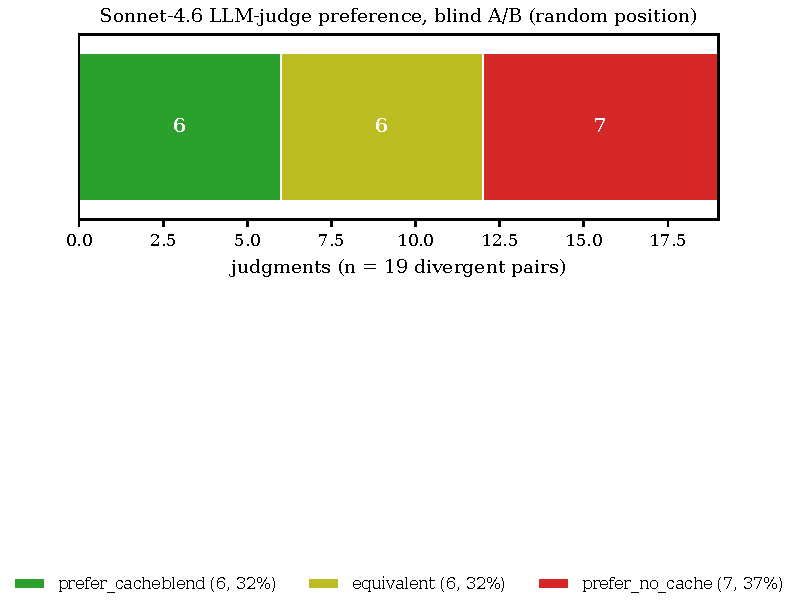
\includegraphics[width=\columnwidth]{figures/judge_summary.pdf}
\caption{Distribution of judge preferences across the 19 divergent
pairs. Equivalent and cacheblend-wins each take 31.6\%; no\_cache-wins
takes 36.8\%. No unparseable judgments.}
\label{fig:judge-summary}
\Description{Horizontal stacked bar chart showing 19 judgments split
into three segments: prefer cacheblend (6, 31.6 percent, green),
equivalent (6, 31.6 percent, olive), and prefer no_cache (7, 36.8
percent, red). No unparseable segment is shown.}
\end{figure}

\paragraph{Per-pair rationales show case-by-case reasoning.}
The per-pair rationales show case-by-case evaluation, not a
mechanical ``prefer tool calls'' heuristic. On
\texttt{swebench\_verified/pytest-7490} turn~3 (no\_cache: tool-call to
a non-existent path; cacheblend: multi-step prose plan), the judge
\emph{prefers cacheblend}: \emph{``Output A provides a more thoughtful,
multi-step plan with multiple relevant tool calls, while Output B
attempts to read a non-existent file path.''} On
\texttt{post\_compact/v6\_align} turn~3, where no\_cache fabricated a
URL-as-filepath while cacheblend ran a working Python demonstration,
the judge again prefers cacheblend. Conversely, on
\texttt{swebench\_verified/astropy-13398} turn~4 (cacheblend: prose
with speculative patch; no\_cache: clean tool call), the judge prefers
no\_cache: \emph{``Output A is a clean, well-formed tool call, while
Output B mixes prose with multiple tool calls and includes a speculative,
likely incorrect patch.''}

The pattern that emerges: cacheblend's blended-KV output is
\emph{sometimes better} than no\_cache's (e.g., when no\_cache picks a
wrong file path and cacheblend's prose plan is more recoverable), but
more often slightly worse, and occasionally catastrophically worse
(the decode-mode flips of \S\ref{sec:eval-identity}). On net, no\_cache
edges cacheblend by 5 percentage points on a 19-pair sample.

\paragraph{Identity rate predicts judge equivalence.} The 28 substantive
bit-identical pairs that we excluded from the judge call (plus the 7
preflight pairs that bypass cacheblend entirely) are trivially
EQUIVALENT; among the 19 judged pairs, the relationship between
token-identity and equivalence persists. All 5 pairs with identity
$\geq$0.5 were judged EQUIVALENT; among the 14 pairs with identity
$<$0.5, the judge returned EQUIVALENT only once. Token-identity is a
strong, near-deterministic predictor of judge equivalence over its
upper half --- below 0.5, real preference signal kicks in. This
matters operationally: a deployment that wants to gate cacheblend
rescue on \emph{measurable} quality preservation can use the
token-identity threshold as a cheap proxy for the judge call, which is
two orders of magnitude more expensive.

\paragraph{Methodological caveats.}
(i) Judge calibration. The multi-judge replication in
Table~\ref{tab:multi-judge} reduces but does not eliminate the
single-judge risk --- all three judges share Anthropic's RLHF
training distribution and could share systematic preferences a
human grader would not have. A human spot-check on a random subset
of the 19 pairs is a sensible next step we do not run here.
(ii) Pairs are dependent (serial sampling within capture), not
independent. The 19 divergent pairs come from 7 captures; pairs from
the same capture share session-cache state, so Wilson CI assumptions
of independence are slightly violated. The CI is reported as-is for
transparency; a clustered bootstrap would tighten it but not change
the headline.
(iii) Conditional vs end-to-end framing. The headline 63.2\% rate is
\emph{conditional} on cacheblend producing a non-bit-identical output
($n_{\text{div}}{=}19$); the end-to-end rate over the 47 substantive
pairs (which folds in the 28 bit-identical pairs as guaranteed
equivalents) is 85.1\%. We do not fold preflight turns back in: rates
of the form $/54$ would mix in pairs where cacheblend never engaged.
(iv) The judge prompt favors tool calls --- intentional calibration to
the agentic context, since CC's wire protocol acts on tool calls and
treats prose as a non-actionable fallback. The judge correctly
preferred prose when the alternative tool call had a wrong
path (pytest-7490 turn~3), suggesting the lean is not pathological.

\subsection{Tool-call vs prose mode agreement}
\label{sec:eval-mode}

A complementary end-to-end view of the agent-protocol cost is whether
the two conditions agree on the model's decode \emph{mode} ---
tool-call (JSON the CC harness can act on) versus prose (which stalls
the agent). For each substantive (capture, turn) pair we classify each
condition's output by whether its first non-whitespace block is a
well-formed function-call JSON. The classifier is a single regex
matching outputs whose leading non-whitespace bytes form a JSON
object containing the keys \texttt{"type": "function"} and
\texttt{"name"}; full regex source is in
\texttt{scripts/dev/extract\_\allowbreak{}tool\_\allowbreak{}call\_\allowbreak{}rate.py}.
This is the same first-block heuristic CC's harness uses to decide
whether to execute a tool call or surface text to the user.

\begin{table}[h]
\small
\centering
\begin{tabular}{lr}
\toprule
Metric over the 47 substantive turns & Rate \\
\midrule
no\_cache tool-call rate              & 30/47 (63.8\%) \\
no\_cache prose rate                  & 17/47 (36.2\%) \\
cacheblend tool-call rate             & 26/47 (55.3\%) \\
cacheblend prose rate                 & 21/47 (44.7\%) \\
\midrule
\textbf{Mode agreement} (NC class $=$ CB class) & \textbf{43/47 (91.5\%)} \\
NC tool-call $\to$ CB prose (\emph{agent stall}) & 4/47 (8.5\%) \\
NC prose $\to$ CB tool-call (recovery) & 0/47 (0.0\%) \\
\bottomrule
\end{tabular}
\caption{Tool-call vs prose mode agreement between no\_cache and
cacheblend, over the 47 substantive pairs of \S\ref{sec:eval-hitrate}'s
corpus. Mode disagreement is \emph{asymmetric}: every disagreement is
cacheblend flipping a tool-call into prose, with no recoveries in the
other direction. The 8.5\% asymmetric stall rate is independent of any
judge-prompt calibration and constitutes a hard floor on cacheblend's
agent-protocol cost on this workload.}
\label{tab:tool-call-mode}
\end{table}

This is the same Mode~A failure mode of \S\ref{sec:eval-identity},
counted directly: blended-KV cacheblend output flips out of tool-call
mode on 4 of the 47 substantive turns where no\_cache would have
produced an actionable tool call. The asymmetry --- zero recoveries
in the prose~$\to$~tool-call direction --- means cacheblend's decode
shift is one-directional and load-bearing for downstream agent
behavior. The 91.5\% mode-agreement rate is consistent with the 85\%
end-to-end non-inferiority rate of \S\ref{sec:eval-judge} (the
difference being that mode agreement counts only protocol form, while
the judge also evaluates argument quality conditional on a matching
mode).

\subsection{Cross-corpus replication on \texttt{skill\_invocation/}}
\label{sec:eval-cross-corpus}

The SWE-V+\texttt{post\_compact} subset (5 SWE-V captures + 2 \texttt{post\_compact/} captures =
$n{=}47$ substantive turns) leaves open whether the findings above
are specific to large-prompt SWE-V-shaped traffic. We replicate the
hit-rate and identity measurements on \dataset's other substantive
subset, \texttt{skill\_invocation/} (1 capture, 53 turns, 52
substantive, max prompt $\sim$2.3k tokens) --- a different workload
shape with shorter prompts and a more uniform skill-preamble
structure. Same backend, same patches, same methodology.

\begin{table*}[t]
\small
\centering
\begin{tabular}{lrrr}
\toprule
Metric & SWE-V+\texttt{post\_compact} subset & \texttt{skill\_inv.} & combined \\
\midrule
$n$ (substantive)              & 47       & 52       & 99 \\
\midrule
\multicolumn{4}{l}{\emph{Rescue rate (\S\ref{sec:eval-hitrate})}} \\
~~median                       & 87.5\%   & 75.4\%   & 76.5\% \\
~~p25                          & 16.1\%   & \textbf{67.9\%} & 67.5\% \\
~~p75                          & 96.8\%   & 95.0\%   & 95.2\% \\
~~$\geq$99\% (steady-state peak) & 6/47 (13\%) & \textbf{0/52 (0\%)} & 6/99 (6\%) \\
~~$\sim$0\% (cold/shift)       & 9/47 (19\%) & 6/52 (12\%) & 15/99 (15\%) \\
\midrule
\multicolumn{4}{l}{\emph{Output identity to no\_cache (\S\ref{sec:eval-identity})}} \\
~~median                       & 1.0000   & 0.8344   & 1.0000 \\
~~bit-identical                & 28/47 (60\%) & 24/52 (46\%) & 52/99 (53\%) \\
~~severe ($<$0.3) divergence   & 14/47 (30\%) & 12/52 (23\%) & 26/99 (26\%) \\
\bottomrule
\end{tabular}
\caption{Same measurements on two \dataset{} subsets and their
union. The qualitative findings replicate; the quantitative shape
of the rescue distribution differs by prompt size in an interpretable
direction.}
\label{tab:cross-corpus}
\end{table*}

\paragraph{What replicates.} The bimodal-with-tail rescue picture,
the order-of-30\% severe-divergence rate, and the
near-50\% bit-identical rate all hold within $\sim$10 percentage
points across the two subsets. The combined-corpus headline numbers
move toward the larger ($n{=}52$) subset's values: median rescue
76.5\%, severe-divergence 26\%, bit-identical 53\%.

\paragraph{What differs by workload shape.} The \texttt{skill\_invocation/}
subset has shorter prompts (max 2.3k tokens vs the SWE-V+\texttt{post\_compact} subset's
4.5--9.5k) and a more uniform within-capture structure (5 skills
$\times$ 3 prompts per skill, cycling). On this workload cacheblend's
rescue distribution \emph{tightens}: the IQR shrinks dramatically
(p25 16.1\%~$\to$~67.9\%) and the steady-state peak vanishes (0/52
turns reach $\geq$99\% rescue, vs 6/47 on §1). The cold-cache tail
also shrinks (19\%~$\to$~12\%). Two structural reasons: (i) shorter
prompts give cacheblend less surface area to either hit perfectly or
miss entirely, so most turns land in the middle band; (ii) the
skill-preamble cycling pattern means each turn's cache LOOKUP tests
against a freshly mixed cache state, never the ``same prompt as
last turn'' steady state where rescue saturates near 100\%.

\paragraph{Implication.} The published 95--99\% cacheblend rescue
peak is not just rare across the SWE-V+\texttt{post\_compact} subset (only 13\% of turns) --- it
appears to be a function of \emph{long, near-duplicate prompts in
sequence}. On workloads dominated by short or structurally-varying
turns it does not appear at all. This sharpens the
``hit rate is not the metric'' thesis: even when rescue \emph{does}
match the published number, it does so on a minority of turns; on
a sibling workload it disappears entirely.

\subsection{Summary}
\label{sec:eval-summary}

The three measurements compose into a single quantitative picture of
cacheblend's tradeoff on Llama-70B fp8 with the \S\ref{sec:patches}
patches:

\begin{itemize}
\item \textbf{Rescue ($n{=}47$ substantive turns):} bimodal --- median
  87.5\%, p25 16.1\%, p75 96.8\%; 13\% of turns reach $\geq$99\%
  steady-state and 19\% sit at $\sim$0\% cold-cache
  (Table~\ref{tab:hit-rate}, Figure~\ref{fig:rescue-distribution}).
\item \textbf{Latency ($n{=}47$):} cacheblend's median TTFT is
  \textbf{55\% slower} than no\_cache (1882\,ms vs 1211\,ms), and
  \textbf{7$\times$ slower} at the $\geq$99\% rescue peak
  (Table~\ref{tab:ttft}, Table~\ref{tab:ttft-by-rescue}). Hit-token
  rescue does not translate to TTFT reduction on this setup.
\item \textbf{Identity ($n{=}47$):} 57\% of substantive turns bit-identical
  to full compute; 30\% diverge severely ($<$0.3 token-identity),
  including 11\% that flip decode mode entirely
  (Figure~\ref{fig:identity-distribution}).
\item \textbf{Agent-protocol usefulness ($n_{\text{div}}{=}19$ divergent
  pairs):} a strong LLM judge prefers cacheblend's output on 31.6\%
  (Wilson CI [15.4\%, 54.0\%]); conditional non-inferiority on the
  divergent pairs is 63.2\%, end-to-end non-inferiority (including the
  28 bit-identical substantive pairs as guaranteed equivalents) is
  85.1\%~/~47 (Table~\ref{tab:judge}, Figure~\ref{fig:judge-summary}).
\item \textbf{Tool-call mode agreement ($n{=}47$):} mode agreement is
  91.5\% but cacheblend asymmetrically flips no\_cache tool-calls into
  prose on 8.5\% of substantive turns (4/47); zero recoveries in the
  other direction (Table~\ref{tab:tool-call-mode}).
\item \textbf{Cross-corpus replication ($n{=}99$, §1 + \texttt{skill\_invocation/}):}
  the bimodal rescue and $\sim$30\% severe-divergence pattern replicates
  on a structurally different second subset, with the $\geq$99\% rescue
  peak vanishing on shorter prompts (0/52 turns on
  \texttt{skill\_invocation/}) and the IQR tightening (p25 jumps
  16\%~$\to$~68\%; Table~\ref{tab:cross-corpus}).
\end{itemize}

Cacheblend's published rescue numbers are reproducible at the
steady-state peak of this distribution but \emph{are not the typical
rescue rate} of natural CC traffic --- the combined-corpus
($n{=}99$) median is 76.5\% with a 15\% cold-cache tail, and the
$\geq$99\% peak appears on only 6\% of turns and is workload-shape
dependent. On the substantive divergent slice where cacheblend's
selective recompute engages non-trivially, the rescued output is
judged non-inferior to a fresh-compute baseline on 63\% of turns,
well below the 85\% spec gate.
\S\ref{sec:discussion} discusses when this trade is acceptable.
